\chapter{Электростатический подвес} \label{chapt1}


\section{Принципы построения электростатических подвесов} \label{sect1_1}

Электростатический подвес представляет собой устройство, удерживающее твердое тело во взвешенном состоянии за счет действия электрических сил, создаваемых системой из конечного количества электродов. Как правило, твердое тело является проводником, а в межэлектродном пространстве поддерживается вакуум.

Как известно \cite{Tamm}, заряд в проводящем теле, находящемся в электрическом поле, распределен таким образом, чтобы внутри тела электрическое поле отсутствовало. Таким образом, на проводник в электрическом поле действуют только поверхностные силы, которые направлены по внешней нормали к поверхности проводника. Величина этих сил невелика, поэтому для увеличения удерживающей силы необходимо увеличивать напряженность. При этом максимальная напряженность поля ограничена электрическим пробоем вакуумного промежутка между поверхностями тела и электродов, значение которого зависит от чистоты проводника, материала проводника, величины достигнутого вакуума и пр.

Электростатические подвесы выполняются как на постоянном, так и на переменном токе. В подвесе на постоянном токе автоматическое изменение напряженности в зазоре между телом и электродами осуществляется по сигналам, пропорциональным изменению емкости между ротором и электродом. В подвесе на переменном токе используется электрический резонанс схемы питания подвеса. Подвесы на резонансных схемах без следящих систем управления напряжением называют пассивными. Активными называются подвесы с следящими системами управления напряжением.


\section{Обзор технических элементов, в которых находит свое применение электростатический подвес. Электростатический гироскоп ЭСГ} \label{sect1_2}
Отсутствие трения является главным достоинством неконтактных подвесов, что позволяет создавать практически «вечные» подшипники, не имеющие проблем износа, шума и ограничений по скорости вращения. Отсюда вытекает множество прикладных решений, построенных на основе таких подвесов. Наиболее распространены неконтактные подвесы в навигации (на рисунке \ref{img:sphere_suspension_photo} – гироскоп с электростатическим подвесом), космической и транспортной отраслях.

\begin{figure}[ht] 
  \centering
  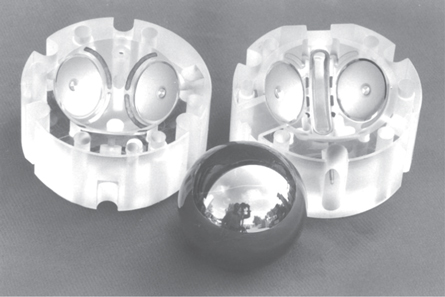
\includegraphics [scale=0.7] {sphere_suspension_photo}
  \caption{Сферический гироскоп с электростатическим подвесом. Фотография ротора и корпуса}
  \label{img:sphere_suspension_photo}
\end{figure}



Основным объектов исследования в работе является электростатический подвес сферического ротора  – основного структурного компонента отечественного электростатического гироскопа ЭСГ, спроектированного в Санкт-Петербургском ЦНИИ «Электроприбор» под руководством главного конструктора А.С. Анфиногенова. ЭСГ – сложнейший гироскопический прибор, работы по которому начались в СССР во второй половине 60-х годов, по сей день является наиболее точным датчиком первичной информации для инерциальных навигационных систем. 

Гироскоп ЭСГ состоит из стеклянной вакуумной камеры, на внутреннюю поверхность которой напылены шесть пар ортогонально расположенных электродов электрического подвеса. Внутри оболочки помещен полый тонкостенный сферической ротор, изготовленный из бериллия. Наружный диаметр ротора составляет 50 мм, вес ротора порядка 20 г, зазор между наружной поверхностью ротора и оболочкой 100 мкм, скорость вращения ротора достигает нескольких тысяч оборотов в минуту. Списывание углового положения ротора осуществляется фотооптическими датчиками \cite{History_ESG}.

К числу наиболее сложных задач, решаемых электростатическими гироскопами, относится навигационное обеспечение атомных подводных лодок, вооруженных баллистическими ракетами большого радиуса действия. Для обеспечения высокой точности ракет необходимо знать навигационные данные подводной лодки на момент старта с точностью на один-два порядка более высокой, чем та, которую обеспечивает навигационное счисление даже на коротких отрезках времени. 
Появление электростатических подвесов дало мощный толчок развитию гироскопической техники, неожиданно открылись совершенно новые интересные задачи \cite{Electropribor}.


%\newpage
%============================================================================================================================


%\newpage
%============================================================================================================================
